
\subsection{SOP details}

\begin{frame}{operations requiring same origin}
    \begin{itemize}
    \item accessing webpage you loaded in iframe, pop-up window, etc.
    \item accessing webpage loading you in iframe, pop-up window, etc.
    \item sending \textit{certain kinds of} requests
        \begin{itemize}
        \item most notably XMLHTTPRequest --- ``AJAX''
        \end{itemize}
    \end{itemize}
\end{frame}

\begin{frame}<1>[label=noSameOrigin]{operations not requiring same origin}
    \begin{itemize}
    \item \myemph<2>{loading images, stylesheets (CSS), video, audio}
    \item \myemph<3>{linking to websites}
    \item \myemph<7>{loading scripts}
        \begin{itemize}
        \item but not getting syntax errors
        \end{itemize}
    \item \myemph<4>{accessing with ``permission'' of other website}
    \item \myemph<5>{submitting forms to other webpages}
    \item \myemph<6>{requesting/displaying other webpages \sout<7>{(but not reading contents)}}
    \end{itemize}
\end{frame}

% FIXME: explanation

\section{information leaks despite SOP}

\againframe<2>{noSameOrigin}

\begin{frame}[fragile,label=inFB]{logged into facebook? (1)}
    \begin{itemize}
        \item \texttt{https://www.facebook.com/login.php?next=\textit{URL}}
        \item login page if \myemph{you are not logged in}
            \item otherwise redirects to \textit{URL}
    \end{itemize}
\end{frame}

\begin{frame}[fragile,label=inFB2]{logged into facebook? (2)}
    \begin{itemize}
        \item \texttt{https://www.facebook.com/favicon.ico} is an image
        \item load via conditional redirect:
    \end{itemize}
    \begin{minted}[fontsize=\small,breaklines,breakafter==]{HTML}
<img src="http://www.facebook.com/login.php?next= https%3A//www.facebook.com/favicon.ico"
    onload="doLoggedInStuff()"
    onerror="doNotLoggedInStuff()">
\end{minted}
    \begin{itemize}
    \item with third-party cookies enabled\ldots (more later)
    \item would work/not work depending on if logged into facebook
    \end{itemize}
\imagecredit{via \texttt{https://robinlinus.github.io/socialmedia-leak/}}
\end{frame}

\againframe<3>{noSameOrigin}

\begin{frame}[fragile,label=visitedLinks]{old problem: visited links}
    \begin{itemize}
    \item browsers can display visited versus unvisited links different:
        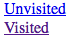
\includegraphics[width=2cm]{../web/visitedunvisited}
    \item javascript can query the ``computed style'' of a link
    \end{itemize}
\begin{minted}[fontsize=\small]{HTML}
<style>:visited{color:red}</style>
<a id="lnk" href="https://facebook.com/secretgroup/">link</a>
<script>
var link = document.getElementById("lnk");
if (window.getComputedStyle(link, null).getProperty('color')
    == ...) {
    ...
}
</script>
\end{minted}
\end{frame}

\begin{frame}[fragile,label=visitedLinksFix]{visited link: fix}
    \begin{itemize}
    \item most browsers have fixed visited link ``leaks'' --- not trivial
    \item getComputedStyle \myemph{lies about visited links}
        \begin{itemize}
        \item as if unvisited
        \end{itemize}
    \item many types of \myemph{formatting disallowed} for visited links
        \begin{itemize}
        \item e.g. different font size --- could detect from sizes of other things
        \end{itemize}
    \item probably \myemph{incomplete solution?}
        \begin{itemize}
            \item still tricks involving page appearance
        \end{itemize}
    \end{itemize}
\end{frame}
